\documentclass{beamer}
\usepackage{beamerthemesplit}
\usepackage{booktabs}
\usepackage{graphicx}
\usepackage{transparent}
\usepackage{bbold}
\usepackage[italian]{babel}
\usepackage[utf8x]{inputenc}
\usepackage{listings}
\usepackage{tikz}
\usetikzlibrary{arrows}
\usepackage{amsmath,amsfonts,amssymb}
\usepackage{pgfplots}
\usepackage{scalefnt}
\usepackage{color}
\usepackage{xcolor}
\usepackage{multicol}
\usepackage{bm}

\title[mRMR]{mRMR - features selection method}
\institute{
\begin{small}
Corso di Laurea in Informatica Magistrale
\end{small}}
\author{\textbf{Simone Rutigliano}}
\date{\tiny{\today}}

\usebackgroundtemplate{
%    \transparent{0.12}{
     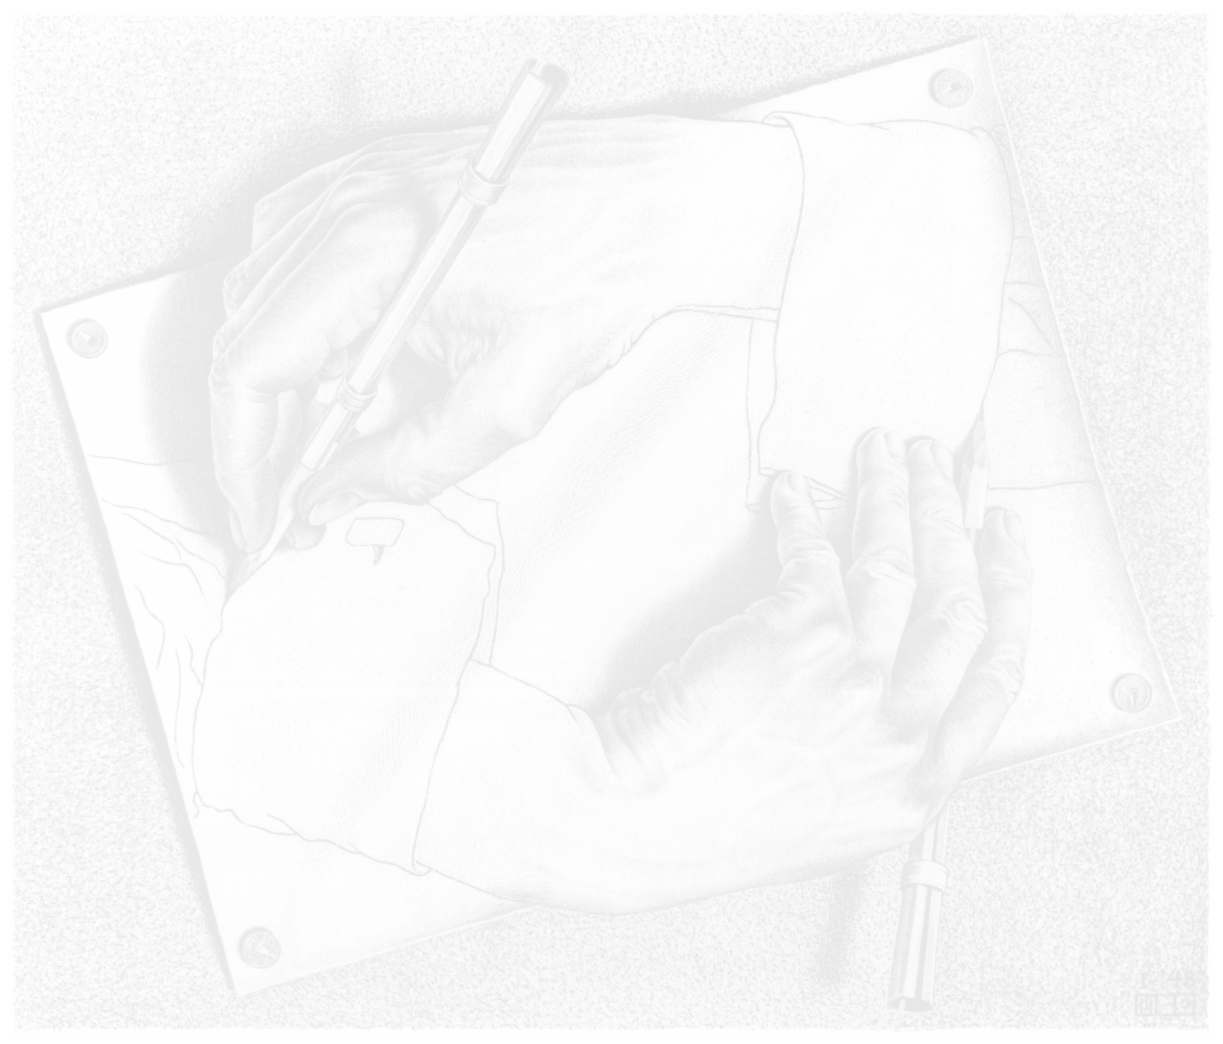
\includegraphics[width=\paperwidth, height=\paperheight]{./figure/theme/escher_hands_tr.png}
%    }
}

%\usetheme{Hannover}
\usetheme{Copenhagen}
\usecolortheme{seahorse}
\usecolortheme{rose}
%\usetheme{Frankfurt}
%\usecolortheme{beetle}

%\useoutertheme[subsection=false]{smoothbars}
%\useoutertheme[subsection=false]{smoothtree}
\useoutertheme{shadow}
\setbeamercovered{dynamic}

\pgfdeclareimage[height=1cm]{logo}{figure/theme/logo}
\logo{\pgfuseimage{logo}}

\begin{document}

%%%%%%%%%%%%%%%%%%%%%%%%%%%%%%%%%%%%%%%%%%%%%%%%%%%%%

\begin{frame}
\maketitle
\end{frame}

%%%%%%%%%%%%%%%%%%%%%%%%%%%%%%%%%%%%%%%%%%%%%%%%%%%%%

\begin{frame}
\frametitle{Outline}
	\begin{multicols}{2}
		\tableofcontents
	\end{multicols}
\end{frame}

%%%%%%%%%%%%%%%%%%%%%%%%%%%%%%%%%%%%%%%%%%%%%%%%%%%%%
\section{Mutual Information}
\subsection{Definizione}
\begin{frame}
	\frametitle{Definizione}
		\nocite{Ding:2003:MRF:937976.938050}
		\nocite{Peng05featureselection}
Date due variabili casuali \emph{X} e \emph{Y} con distribuzione di probabilità congiunta $p(x, y)$, la mutua
informazione è definita come \\~$$I(X; Y ) = H(X) − H(X|Y ) = H(Y ) − H(Y |X)$$\\~\\
La mutua informazione rappresenta i bit di informazione che una delle variabili fornisce circa l'altra
\begin{figure}[htb]
	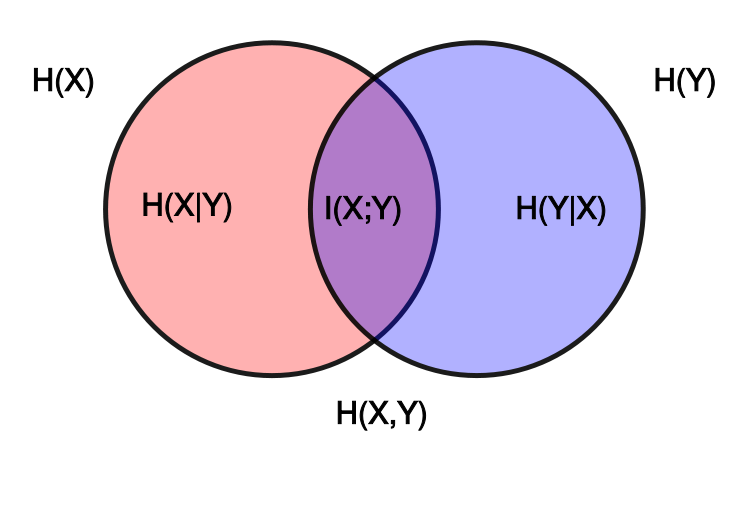
\includegraphics[width=0.50\textwidth]{figure/mutual.png}
\end{figure}
\end{frame}
\begin{frame}
	\frametitle{Considerazioni}
	\begin{itemize}
		\item $I(X;Y)=0 \Rightarrow$ \emph{X} e \emph{Y} sono variabili indipendenti
		\item $\pmb{I(X;Y)} = H(X)-H(X|Y)=H(Y)-H(Y|X)= \pmb{I(Y;X)}$
		\item $I(X;X)=H(X)$
	\end{itemize}
\end{frame}
\begin{frame}
	\frametitle{Esempio}
	Lanciamo 10 monete:
	\begin{itemize}
		\item \emph{X} rappresenta i valori delle prime 7 monete
		\item Y quelli delle ultime 5
	\end{itemize}
	Avremo che:
	\begin{columns}
		\begin{column}{0.5\textwidth}
			\begin{itemize}
				\item $H(X) = 7$
				\item $H(Y) = 5$\newline
			\end{itemize}
		\end{column}
		\begin{column}{0.5\textwidth}
			\begin{itemize}
				\item $H(X|Y) = 5$
				\item $H(Y|X) = 3$\newline
			\end{itemize}
		\end{column}
	\end{columns}
	La mutua informazione sarà quindi pari a
$$I(X; Y ) = I(Y ; X) = 2 $$
\end{frame}
\subsection{Formule}
\begin{frame}
	\frametitle{Discrete}
	Definite due variabili casuali discrete \emph{X} e \emph{Y}
	$$ I (x;y) = \sum\limits_{y \in Y} \sum\limits_{x \in X} p(x,y)\log \frac{p(x,y)}{p(x)p(y)}$$
	dove
	\begin{itemize}
		\item $p(x,y)$ è la funzione di distribuzione di probabilità congiunta di \emph{X} e \emph{Y}
		\item $p(x)$ e $p(y)$ sono le funzioni di distribuzione di probabilità marginale di X e Y
	\end{itemize}
\end{frame}
\begin{frame}
	\frametitle{Continuous}
	$$ I (x;y) = \int_Y \int_X p(x,y)\log \frac{p(x,y)}{p(x)p(y)} \mathrm{d}x \mathrm{d}y$$
	dove
	\begin{itemize}
		\item $p(x,y)$ è la funzione di densità di probabilità congiunta di \emph{X} e \emph{Y}
		\item $p(x)$ e $p(y)$ sono le funzioni di densità di probabilità marginale di X e Y
	\end{itemize}
\end{frame}
\subsection{Problematiche}
\begin{frame}
	\frametitle{Problematiche}
	\begin{itemize}
		\item In caso di variabili continue, difficoltà nella computazione degli integrali nello spazio continuo su un numero limitato di campioni
	\end{itemize}
	\textbf{Soluzione}
	\begin{itemize}
		\item Incorporare la discretizzazione dei dati nella fase di preprocessing
	\end{itemize}
\end{frame}

%%%%%%%%%%%%%%%%%%%%%%%%%%%%%%%%%%%%%%%%%%%%%%%%%%%%%

\section{Max Dependency}
\subsection{Definizione}
\begin{frame}
	\frametitle{Max Dependency \dots}
	In termini di mutua informazione, l'obiettivo è trovare il set di feature \emph{S} con \emph{m} features che hanno la più alta dipendenza con la classe target \emph{c}
	$$ \max Dep(S,c)~~~~~ Dep = I(\{x_1,\dots,x_m \};c )$$
	Dove 
	\begin{itemize}
		\item $x_1,\dots,x_m$ sono le $m$ features selezionate
		\item $I$ indica la mutua informazione tra le feature del set
	\end{itemize}
\end{frame}

\subsection{Formula}
\begin{frame}
	\frametitle{\dots Max Dependency}
	\begin{itemize}
		\item Dato un set contenente \emph{m-1} features( $S_{m-1}$) l'\emph{m-}sima feature consiste  nella feature che più riesce ad incrementare la mutua informazione $I(S,c)$
	\end{itemize}
	\begin{align*}
	I (S_m;c) &= \int\int p(S_m,c)\log \frac{p(S_m,c)}{p(S_m)p(c)} \mathrm{d}S_m \mathrm{d}c \\
	&= \int\int p(S_{m-1},x_m,c)\log \frac{p(S_{m-1},x_m,c)}{p(S{m-1},x_m)p(c)} \mathrm{d}S_{m-1}\mathrm{d}S_m\mathrm{d}c \\
	&=\int\dots\int p(x_1,\dots,x_m,c)\log \frac{p(x_1,\dots,x_m,c)}{p(x_1,\dots,x_m)p(c)} \mathrm{d}x_1,\dots,\mathrm{d}x_m \mathrm{d}c \\\\
	\end{align*}

\end{frame}

\subsection{Problemi}
\begin{frame}
	\frametitle{Problemi nel continuo}
	Difficoltà nella stima accurata delle funzioni di densità multivariate $p(x_1,\dots,x_m)$ e $p(x_1,\dots,x_m,c)$
	\begin{itemize}
		\item Numero di campioni insufficienti
		\item Comporta il calcolo delle inverse delle matrice di covarianza multidimensionali
		\item Computazione molto lenta
	\end{itemize}
\end{frame}

\begin{frame}
	\frametitle{Problemi nel discreto}
	Difficoltà nel calcolo delle funzioni di distribuzione di probabilità congiunta $p(x_1,\dots,x_m)$ e $p(x_1,\dots,x_m,c)$
	\begin{itemize}
		\item Numero di campioni insufficienti
		\item Computazione molto lenta in caso di un valore \emph{m} molto alto
	\end{itemize}
\end{frame}

\begin{frame}
	\frametitle{Soluzione}
	\begin{itemize}
		\item Approssimare la funzione di dipendenza ad una funzione computazionalmente meno onerosa
	\end{itemize}
\end{frame}

%%%%%%%%%%%%%%%%%%%%%%%%%%%%%%%%%%%%%%%%%%%%%%%%%%%%%

\section{Max Relevance}
\subsection{Definizione}
\begin{frame}
	\frametitle{Max Relevance - Definizione}
	\begin{itemize}
		\item Ricercare le feature che riescano ad approssimare la funzione 	$$ \max Dep(S,c)~~~~~ Dep = I(\{x_1,\dots,x_m \};c )$$
		con il valor medio di tutti i valori della mutua informazione tra le singole feature $x_i$ e la classe $c$
	\end{itemize}
\end{frame}
\subsection{Formule}
\begin{frame}
	\frametitle{Per variabili discrete}
	In caso di variabili discrete l'obiettivo sarà massimizzare la funzione \emph{Dep} calcolata nel seguente modo
	$$Dep= \frac{1}{|S|} \sum\limits_{x_i \in S} I (x_i;c)$$
	dove 
	\begin{itemize}
		\item S indica il set contenente tutte le features
		\item $x_i$ indica la \emph{i-}sima feature da considerare
		\item $c$ indica la classe target
	\end{itemize}
\end{frame}

\begin{frame}
	\frametitle{Per variabili continue\dots}
	Per le variabili continue bisogna usare la \emph{F-}statistic come misura per calcolare la rilevanza tra le features $x_i$ e la classe target \emph{c}
	$$ F(x_i,c) = \frac{\frac{\sum\limits_{K}{n_k(\bar{x_k}-\bar{x})}}{K-1}}{\sigma^2}$$
	dove: 
	\begin{itemize}
		\item $\sigma^2=\frac{ \sum\limits_{k}{(n_k-1)\sigma^2_k}}{n-K}$
		\item $k$ indica le classi denotate da $c$
		\item $\bar{x}$ è il valor medio di $x_i$ di tutti i campioni
		\item $\bar{x_k}$ è il valor medio di $x_i$ di tutti i campioni di classe $k$
		\item $n_k$ e $\sigma_k$ indicano dimensione e varianza della $k-$classe
	\end{itemize}
\end{frame}

\begin{frame}
	\frametitle{\dots per variabili continue}
	In caso di variabili continue l'obiettivo sarà massimizzare la funzione \emph{Dep} calcolata nel seguente modo
	$$Dep= \frac{1}{|S|} \sum\limits_{x_i \in S} F(x_i;c)$$
	dove 
	\begin{itemize}
		\item $F$ indica la funzione $F-test$ calcolata sulle feature in relazione alla classe target
		\item $S$ indica il set contenente tutte le features
		\item $x_i$ indica la \emph{i-}sima feature da considerare
		\item $c$ indica la classe target
	\end{itemize}
\end{frame}

\subsection{Problematiche}
\begin{frame}
	\frametitle{Problematiche}
	\begin{itemize}
		\item Features selezionate in questo modo potrebbero essere ricche di \textbf{ridondanza}\newline
		\item Se due features dipendono l'una dall'altra è probabile che eliminando una di esse il potere discriminante non sarà decrementato
	\end{itemize}
\end{frame}

%%%%%%%%%%%%%%%%%%%%%%%%%%%%%%%%%%%%%%%%%%%%%%%%%%%%%
\section{Min Redundancy}
\subsection{Definizione}
\begin{frame}
	\frametitle{Min Redundancy - Definizione}
	\begin{itemize}
		\item Consiste nel selezionare le features in modo tale che siano tra loro più dissimilari possibili
		\item Il subset che si otterrà sarà il più rappresentativo possibile dell'intero dataset
	\end{itemize}
	Formalmente consiste nel 
	\begin{itemize}
	\item Calcolare una funzione \textbf{Red} calcolata sul set di feature $S$
	\item Trovare il subset che minimizza la funzione calcolata
	\end{itemize}
	$$\min Red(S)$$
\end{frame}

\subsection{Formule}
\begin{frame}
	\frametitle{Per variabili discrete}
	$$Red (S)= \frac{1}{|S|^2} \sum\limits_{x_i,x_j \in S} I (x_i;x_j)$$
	dove 
	\begin{itemize}
		\item $|S|(= m)$ è il numero di features presenti nel subset $S$
		\item $x_i$ e $x_j$ rappresentano rispettivamente la $i$-esima e $j$-esima feature del subset $S$
		\item $I (x_i;x_j)$ rappresenta la mutua informazione tra le due feature
	\end{itemize}
\end{frame}

\begin{frame}
	\frametitle{Per variabili continue}
	$$Red(S)= \frac{1}{|S|^2} \sum\limits_{x_i,x_j \in S} |c (x_i;x_j)|$$
	dove 
	\begin{itemize}
		\item $|S|(= m)$ è il numero di features presenti nel subset $S$
		\item $x_i$ e $x_j$ rappresentano rispettivamente la $i$-esima e $j$-esima feature del subset $S$
		\item $|c (x_i;x_j)|$ indica il valore assoluto del coefficiente di correlazione di Pearson tra le feature $x_i$ e $x_j$
	\end{itemize}
\end{frame}

%%%%%%%%%%%%%%%%%%%%%%%%%%%%%%%%%%%%%%%%%%%%%%%%%%%%%

\section{mRMR}
\subsection{Definizione}
\begin{frame}
	\frametitle{mRMR - Definizione}
	Based on these observations, we propose to expand the representative power of
	the feature set by requiring that features are maximally dissimilar to each other,
	for example, their mutual Euclidean distances are maximized, or their pair-wise
	correlations are minimized. These minimum redundancy criteria are supplemented
	by the usual maximum relevance criteria such as maximal mutual information with
	the target phenotypes. We therefore call this approach the minimum redundancy —
	maximum relevance (MRMR) approach.
\end{frame}

\subsection{Formule}
\begin{frame}
	\frametitle{Calcolo mRMR}
	\begin{itemize}
		\item Variabili discrete
			\begin{itemize}
				\item MID - Mutual information difference
				\item MIQ - Mutual information quotient\newline
			\end{itemize}
		\item Variabili continue
			\begin{itemize}
				\item FCD - F-test correlation difference
				\item FCQ - F-test correlation quotient
			\end{itemize}
	\end{itemize}
\end{frame}
\begin{frame}
	\frametitle{Discrete - MID}
	$$\max \Phi(D,R), \Phi = D - R$$
	dove $D=I(i,h)$ e $R=\frac{1}{|S|}\sum\limits_{j \in S}I(i,j)$
\end{frame}

\begin{frame}
	\frametitle{Discrete - MIQ}
	$$\max \Phi(D,R), \Phi = \frac{D}{R}$$
\end{frame}
\begin{frame}
	\frametitle{Continuous}
\end{frame}
\begin{frame}
	\frametitle{Continuous - FCD}
\end{frame}

\begin{frame}
	\frametitle{Continuous - FCQ}
\end{frame}

\subsection{Benefici}
\begin{frame}
	\frametitle{Benefici}
	The benefits of this approach can be real-
	ized in two ways. (1) With the same number of features, we expect the MRMR
	feature set to be more representative of the target phenotypes, therefore leading to
	better generalization property. (2) Equivalently, we can use a smaller MRMR fea-
	ture set to effectively cover the same space as a larger conventional feature set does.
\end{frame}
%%%%%%%%%%%%%%%%%%%%%%%%%%%%%%%%%%%%%%%%%%%%%%%%%%%%%

\begin{frame}{Bibliography}
	\frametitle{References}
	\bibliographystyle{alpha}
	\bibliography{mybib}
\end{frame}
\end{document}
